\section{Results}

\subsection{Dataset and Evidence Provenance}

The final evidence bundle included all 15 apps with static and runtime build-aligned evidence, and no app was classified as a true evidence hole. Table~\ref{tab:cutoff-evidence-summary} reports the selected runtime evidence by app and evidence class. Counts represent build-aligned runs selected from the 14-day evidence window. Full app versions, APK hashes, static and dynamic run identifiers, and alignment records are retained in the generated source bundle. Results therefore refer to selected package/version groups rather than mutable installed-app state.

\begin{table*}[!t]
\centering
\caption{Selected 14-day evidence bundles and provenance.}
\label{tab:cutoff-evidence-summary}
\scriptsize
\begin{tabular}{lllc}
\toprule
App & Category & Version & I/Q/Int \\
\midrule
BBC News & News & 2026.5.0 & 4/0/6 \\
CNN & News & 26.13.0 & 4/1/7 \\
The Guardian & News & 6.226.23011 & 3/2/4 \\
Facebook & Social Media & 567.1.0.52.74 & 3/1/4 \\
Instagram & Social Media & 436.0.0.41.73 & 2/4/1 \\
Pinterest & Social Media & 14.26.0 & 5/0/2 \\
Reddit & Social Media & 2026.26.0 & 2/3/1 \\
Snapchat & Social Media & 14.14.0.43 & 1/2/2 \\
TikTok & Social Media & 45.7.3 & 0/8/3 \\
X & Social Media & 12.5.0-release.0 & 3/1/4 \\
Facebook Msg & Messaging & 567.1.0.53.87 & 4/0/5 \\
Signal & Messaging & 8.18.2 & 3/0/4 \\
Telegram & Messaging & 12.8.3 & 3/0/4 \\
WhatsApp & Messaging & 2.26.25.80 & 4/0/5 \\
LinkedIn & Prof. Networking & 4.1.1218 & 3/1/4 \\
\bottomrule
\end{tabular}
\vspace{1pt}
\begin{flushleft}\scriptsize Categories reflect primary application function rather than corporate ownership or every supported feature.\end{flushleft}
\end{table*}


\subsection{Static Exposure Across Selected Builds}

Static exposure varied substantially across the selected builds. Fig.~\ref{fig:static-exposure} compares three indicators at the manuscript-level: high- and medium-severity finding volume, unguarded-export findings, and dangerous permissions. High- and medium-severity findings ranged from 16 for BBC News and Pinterest to 325 for Snapchat. Facebook and Instagram also exhibited comparatively large finding volumes, with 164 and 128 findings, respectively. A similar concentration appeared in unguarded-export findings: Snapchat had 308, Facebook had 118, and Instagram had 91. Dangerous-permission counts were less dispersed, with several messaging and social apps clustered between 18 and 20.

Across all selected builds, the static export contained 1,235 high/medium findings and 955 unguarded-export findings. The median app had 52 high/medium findings and 45 unguarded-export findings, so the largest apps are not only marginally higher; they dominate the upper tail. Platform-aligned findings closely track the high/medium totals, while network-security findings are much smaller in count, ranging from 0 to 6 per app. These values represent descriptive exposure counts rather than calibrated exploitability or compliance scores, and the complete seven-metric static table is retained in the generated report bundle.

\begin{figure}[!t]
\centering
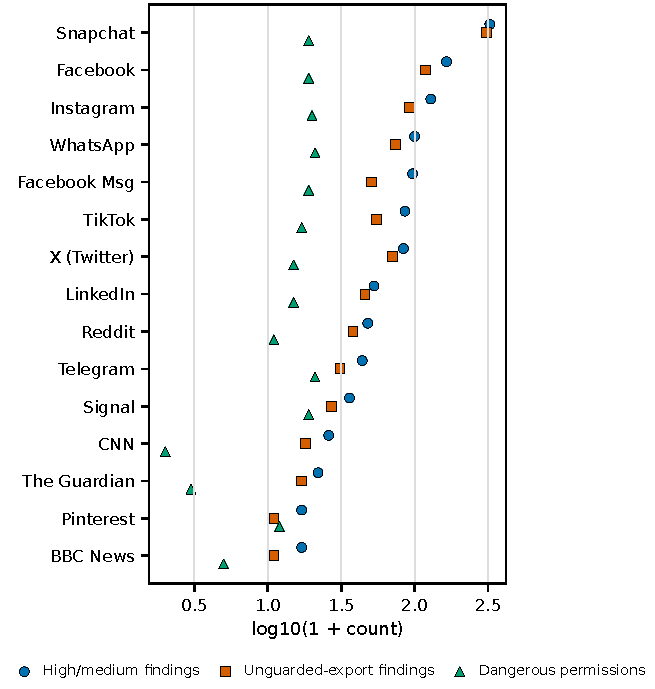
\includegraphics[width=\columnwidth]{figures/fig2_static_exposure_dotplot.pdf}
\caption{Static exposure indicators for the selected app builds. Counts are shown on a logarithmic scale to compare high/medium findings, unguarded-export findings, and dangerous permissions.}
\label{fig:static-exposure}
\end{figure}

\subsection{Runtime Coverage and Behavioral Variation}

The selected runtime evidence includes strict-idle, QFG, and interactive captures. Table~\ref{tab:runtime-behavior-summary} reports compact behavior indicators, while Fig.~\ref{fig:runtime-coverage} shows the distribution of evidence classes across the dataset. QFG is retained as a separate class because a foregrounded but untouched app may continue loading content, synchronizing services, or maintaining communication state. Treating such activity as strict-idle would overstate baseline quietness.

The selected runtime bundle contains 123 dynamic runs: 44 strict-idle, 23 QFG, and 56 interactive captures. CNN and BBC News provide the deepest selected coverage, with 12 and 10 runs, respectively, and every app contributes at least five selected runs. Interaction produced clearer changes in packet rate and traffic volume than in retained hostname count. TikTok, Instagram, WhatsApp, and Facebook exhibited some of the largest interactive packet-rate or traffic-volume measurements. Signal and Telegram showed substantial packet-rate increases from comparatively quiet baselines, while retaining narrower observed hostname breadth under the exercised messaging scenarios.

The runtime results separate activity volume from retained-name breadth. Interactive packet rates ranged from 14.0 packets/s for The Guardian to 285.7 packets/s for TikTok, with a median of 41.6 packets/s. Interactive median transfer volume ranged from about 10.1 MB for Facebook Messenger to 211.3 MB for Instagram. Hostname breadth was less dispersed: the median interactive retained-host count was 12, and most content apps clustered between 10 and 16 hosts. Messaging apps therefore require a different interpretation: WhatsApp, Signal, and Telegram show large baseline-relative packet-rate shifts, but only three or fewer interactive hosts in the selected captures. A zero retained-hostname value does not imply an absence of network traffic; packet activity may occur without a retained DNS/SNI hostname observation.

\begin{table*}[t]
\centering
\caption{Runtime coverage and median behavior indicators.}
\label{tab:runtime-behavior-summary}
\tiny
\begin{tabular}{lrrcrrrr}
\toprule
App & Runs & I/Q/Int & Idle domains & Int domains & Idle pps & Int pps & Int MB \\
\midrule
BBC News & 10 & 4/0/6 & 15 & 16 & 5.8 & 36.1 & 35.8 \\
CNN & 12 & 4/1/7 & 12 & 14 & 5.9 & 34.9 & 34.2 \\
The Guardian & 9 & 3/2/4 & 11 & 14 & 7.6 & 14.0 & 16.5 \\
Facebook & 8 & 3/1/4 & 12 & 16 & 6.2 & 145.5 & 174.4 \\
Instagram & 7 & 2/4/1 & 10 & 15 & 9.7 & 212.5 & 211.3 \\
Pinterest & 7 & 5/0/2 & 7 & 10 & 2.1 & 31.0 & 17.8 \\
Reddit & 6 & 2/3/1 & 11 & 12 & 6.9 & 41.6 & 10.6 \\
TikTok & 11 & 0/8/3 &  & 14 &  & 285.7 & 203.8 \\
X & 8 & 3/1/4 & 11 & 12 & 2.1 & 18.1 & 20.5 \\
LinkedIn & 8 & 3/1/4 & 9 & 10 & 5.4 & 84.5 & 86.3 \\
Signal & 7 & 3/0/4 & 1 & 3 & 0.4 & 95.8 & 33.0 \\
Snapchat & 5 & 1/2/2 & 11 & 11 & 4.0 & 30.2 & 50.9 \\
Telegram & 7 & 3/0/4 & 1 & 0 & 0.7 & 61.5 & 15.2 \\
WhatsApp & 9 & 4/0/5 & 2 & 3 & 0.6 & 207.0 & 153.5 \\
Facebook Messenger & 9 & 4/0/5 & 4 & 9 & 1.5 & 30.1 & 10.1 \\
\bottomrule
\end{tabular}
\end{table*}


\begin{figure}[!t]
\centering
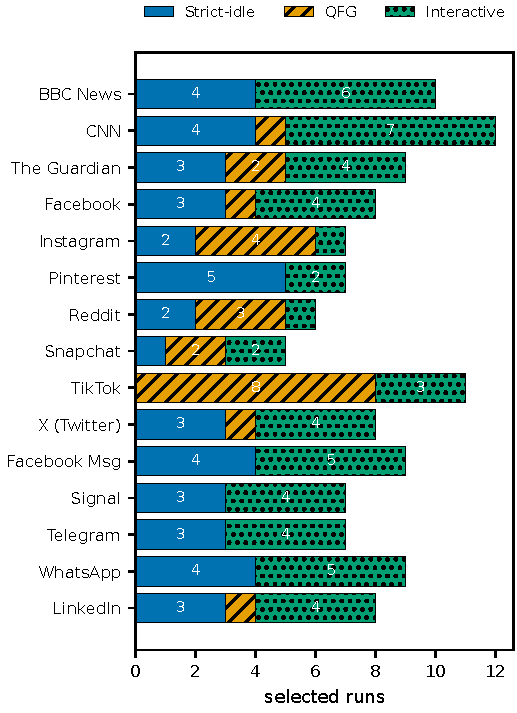
\includegraphics[width=\columnwidth]{figures/fig3_runtime_coverage_by_app.pdf}
\caption{Selected runtime evidence by app. Strict-idle, QFG, and interactive captures are reported separately.}
\label{fig:runtime-coverage}
\end{figure}

\subsection{Integrated Static--Runtime Findings}

The integrated analysis uses a transparent median split rather than an opaque composite score. Table~\ref{tab:integrated-profile-matrix} groups apps by higher or lower static exposure and higher or lower runtime activity, using high/medium finding volume and interactive retained-host count. Higher static exposure denotes at least 52 high/medium findings, and higher runtime activity denotes at least 12 interactive hosts; ties are assigned to the higher group. The four cells are cohort-relative evidence/posture groups: high static / lower runtime indicates packaged exposure not strongly expressed as retained-name breadth in the sampled scenarios; lower static / higher runtime indicates active communication that is not matched by high detector volume.

These groupings are descriptive. Static exposure and runtime activity measure different properties, and disagreement between them is itself informative for review. Four apps fall into the high-static/high-runtime group, four into high-static/lower-runtime, four into lower-static/high-runtime, and three into lower-static/lower-runtime.

\begin{table}[!t]
\centering
\caption{Cohort-relative static--runtime profiles.}
\label{tab:integrated-profile-matrix}
\footnotesize
\setlength{\tabcolsep}{3pt}
\renewcommand{\arraystretch}{1.14}
\begin{tabularx}{\columnwidth}{@{}>{\raggedright\arraybackslash}p{0.22\columnwidth}>{\raggedright\arraybackslash}p{0.27\columnwidth}>{\raggedright\arraybackslash}X@{}}
\toprule
Profile & Cohort-relative criterion & Apps \\
\midrule
\textbf{Lower on both} ($n=3$) & Findings $<52$; hosts $<12$ & Pinterest, Signal, Telegram \\
\textbf{Runtime-broad} ($n=4$) & Findings $<52$; hosts $\geq 12$ & BBC News, CNN, The Guardian, Reddit \\
\textbf{Static-heavy} ($n=4$) & Findings $\geq 52$; hosts $<12$ & Snapchat, Messenger, WhatsApp, LinkedIn \\
\textbf{Higher on both} ($n=4$) & Findings $\geq 52$; hosts $\geq 12$ & Facebook, Instagram, TikTok, X \\
\bottomrule
\end{tabularx}
\par\vspace{3pt}
\noindent\parbox{\columnwidth}{\footnotesize Findings denote high/medium finding volume; hosts denote interactive retained DNS/SNI hostname breadth. Thresholds are cohort medians, and profiles are descriptive rather than risk ratings.}
\end{table}


\begin{figure*}[!t]
\centering
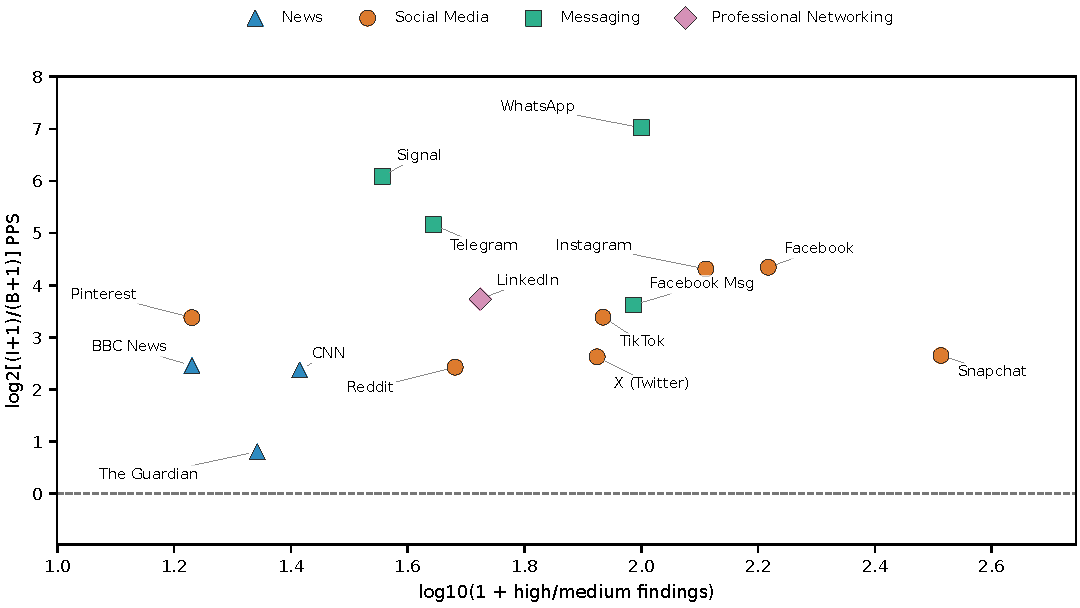
\includegraphics[width=0.88\textwidth]{figures/fig4_static_runtime_scatter.pdf}
\caption{Static exposure and baseline-relative runtime change for selected app builds. Static exposure is the $\log_{10}(1+x)$ transformation of high/medium finding count. Runtime change is $\log_2[(I+1)/(B+1)]$, the additive-smoothed interactive-to-baseline packet-rate ratio, where baseline $B$ is the strict-idle median if present and the QFG median otherwise. Categories reflect primary app function; labeled points identify representative cases discussed in the text.}
\label{fig:static-runtime-scatter}
\end{figure*}

\subsection{App-Level Divergence and Representative Cases}

Several apps illustrate why static and runtime evidence should be interpreted together. Snapchat is the clearest static-heavy case: its selected build has the largest static finding volume, while its interactive retained-host median (11) sits just below the cohort runtime cutoff of 12. Facebook combines high static exposure with broad observed runtime hostname activity. CNN and BBC News exhibit lower static finding volumes than the large social platforms but show clear interactive broadening and substantial runtime evidence depth.

Messaging apps provide a different pattern. Signal and Telegram exhibit comparatively narrow observed hostname breadth, yet both show pronounced packet-rate changes relative to quiet baselines. WhatsApp similarly demonstrates a large baseline-relative packet-rate increase despite a smaller interactive host count than content-feed apps. TikTok and Instagram combine elevated static exposure with substantial runtime activity under the selected scenarios.

Fig.~\ref{fig:static-runtime-scatter} illustrates these differences. The absence of a simple one-to-one relationship is not contradictory; rather, it demonstrates that static exposure and runtime behavior characterize different dimensions of the same selected app builds. Apps may therefore appear static-heavy, runtime-heavy, elevated across both layers, or comparatively limited in both measured dimensions.

The near-zero descriptive association between high/medium static findings and interactive retained-host count in Table~\ref{tab:statistical-summary} should be read in that context. Excluding Snapchat, the near-zero monotonic association persists, so the cohort-level result is not an artifact of the largest static outlier. A static detector count captures declared components, permissions, packaged configuration, and detector posture; an interactive host count captures observed retained DNS/SNI breadth during selected scenarios. The weak app-level association is therefore not a negative result. It shows that a static-only table would miss runtime-heavy apps, while a runtime-only table would miss packaged exposure in static-heavy apps.

Baseline-relative runtime comparisons were audited at the app level before reporting. The generated eligibility export records baseline/QFG and interactive availability for every selected app; in this bundle, all 15 apps have both baseline-side and interactive-side evidence. This prevents aggregate shift summaries from being interpreted beyond the app-level eligibility recorded in the source data.

\begin{table}[!t]
\centering
\caption{Compact descriptive statistical summary.}
\label{tab:statistical-summary}
\scriptsize
\begin{tabular}{@{}p{0.42\columnwidth}p{0.34\columnwidth}r@{}}
\toprule
Measure & Basis & Value \\
\midrule
Selected apps & Build-aligned set & 15 \\
Selected dynamic runs & QA-valid runs & 123 \\
Strict idle/QFG/interactive & Evidence classes & 44/23/56 \\
Runtime-shift eligible apps & Baseline+interactive & 15 \\
Median smoothed log2 PPS shift & App medians & 3.39 \\
Spearman rho, findings vs. hosts & n=15 / n=14 excl. Snapchat & 0.01 / 0.04 \\
\bottomrule
\end{tabular}
\vspace{1pt}
\begin{flushleft}\scriptsize Runtime shift is $\log_2[(I+1)/(B+1)]$ using strict-idle when available, otherwise QFG. Associations are descriptive rank correlations.\end{flushleft}
\end{table}

